%!TEX root = ./template-skripsi.tex
%-------------------------------------------------------------------------------
% 								BAB I
% 							LATAR BELAKANG
%-------------------------------------------------------------------------------

\chapter{PENDAHULUAN}

\section{Latar Belakang Masalah}

Saat ini internet merupakan suatu kebutuhan bagi masyarakat secara umum yang berimplikasi terhadap jumlah situs yang terdapat pada \textit{World Wide Web}. Berdasarkan survei yang dilakukan NetCraft pada bulan April tahun 2022, terdapat 1 miliar situs yang terdapat di web dengan 202 juta situs yang aktif. Dengan banyaknya situs tersebut, maka pengguna internet memerlukan sebuah mesin pencari.

Mesin pencari atau yang biasa disebut \emph{Search Engine} merupakan sebuah program komputer yang berguna untuk membantu pengguna dalam mencari situs web berdasarkan permintaan pencarian pengguna. Mesin pencari sebenarnya tidak berbeda dengan \textit{website} pada umumnya, hanya saja perannya lebih terfokus pada pengumpulan dan pengorganisasian berbagai informasi di internet sesuai dengan kebutuhan penggunanya. Selain untuk memudahkan pencarian, mesin pencari juga berguna untuk meningkatkan pengunjung sebuah situs web.

Mesin pencari pertama kali diperkenalkan oleh Alan Emtage pada tahun 1990 dengan nama \textit{Archie}. \textit{Archie} melakukan pengindeksan \textit{file} pada web dan hanya dapat menampilkan daftar nama situs, tidak dengan isi atau kontennya \citep{seymour2011history}. Setelah kemunculan \textit{Archie}, di tahun berikutnya mulai bermunculan mesin pencari baru. Pada tahun 1993 \textit{Aliweb} muncul dengan memberikan kesempatan pengguna untuk mengunggah halaman situsnya agar terindeks dan memberikan deskripsi untuk halaman tersebut. Kemudian \textit{Altavista} muncul pada tahun 1995 yang menggunakan teknik dan algoritma yang lebih maju. Setelah \textit{Altavista}, pada 2004 muncullah \textit{Yahoo} sebagai salah satu mesin pencari yang maju di mana pengelola dan pemilik situs dapat menambah dan mengedit informasi dalam web tanpa mengeluarkan biaya. Namun, perkembangan mesin pencarian \textit{Yahoo} sangat lambat sehingga pengguna internet perlahan mulai mencari mesin pencari yang lain \citep{seymour2011history}.

\textit{Search engine} yang saat ini paling banyak digunakan adalah \textit{Google}. Mesin pencari yang diluncurkan pada tahun 1998 ini berkembang jauh berbeda dengan mesin pencari yang lain. Mereka mampu mengindeks halaman-halaman dan melakukan perangkingan, yang berarti bahwa halaman yang paling sering dikunjungi atau diklik akan berada paling atas dalam pencarian dengan \textit{keyword} terkait.

\textit{Search engine} dalam perkembangannya tidak hanya memuat halaman berisi informasi, namun juga dapat menjadi sarana iklan. Pada mesin pencari \textit{Google}, terdapat layanan iklan yang disebut dengan \textit{Adwords}. Layanan ini memungkinkan untuk pemilik usaha untuk mengiklankan situs web usahanya, sehingga saat pengguna Google mencari suatu barang, hasil pencarian \textit{Google} akan menampilkan situs web pemilik usaha di bagian teratas dan tertulis sebagai "Ad" atau iklan.

Dalam arsitektur pembuatan \textit{search engine}, terdapat salah satu bagian yang disebut \textit{crawler}. \textit{Crawler} berfungsi untuk mengumpulkan data-data yang akhirnya data-data tersebut akan diproses dan ditampilkan ke pengguna. \textit{Crawler} ini perlu dirancang sebaik mungkin untuk mengumpulkan data yang dapat mendukung \textit{search engine}.

\textit{Web crawler} pertama kali dimunculkan pada tahun 1944 bernama \textit{RBSE} dengan dasar dua program yaitu \textit{Spider} dan \textit{Mite} \citep{eichmann1994the}. Dua program dasar ini berguna untuk membentuk antrian data dalam \textit{database} serta untuk mengunduh halaman dari sebuah web. Guna dari \textit{web crawler} sendiri adalah sebagai perangkat lunak yang secara otomatis bekerja untuk menjelajahi \textit{website} dengan cara terorganisir.

\textit{Web crawler} berperan penting pada \textit{search engine} karena berfungsi untuk mengumpulkan data sebanyak-banyaknya. Tanpa \textit{web crawler}, \textit{search engine} tidak akan mempunyai data dan tidak bisa melakukan \textit{indexing}. Data yang dihasilkan dari sebuah \textit{web crawler} ini adalah data yang terbaru dan memiliki nilai keakuratan yang tinggi. \textit{Web crawler} yang dimiliki \textit{Google} bernama \textit{Googlebot}, \textit{web crawler} \textit{Bing} bernama \textit{Bingbot}, dan \textit{web crawler} \textit{Yahoo} bernama \textit{Slurp bot}.

Dalam jurnal tahun 2020 oleh Kaur dan Geetha, mereka membuat sebuah \textit{web crawler} untuk \textit{hidden web} menggunakan \textit{SIM+HASH} disertai dengan \textit{Redis Server} \citep{kaur2020simhar}. \textit{Web crawler} ini mampu menghasilkan hasil halaman dengan tingkat kecocokan yang maksimum. Meski hasil yang ditampilkan sangat relevan dengan \textit{keyword} yang dimasukkan, namun dalam pembangunannya, \textit{web crawler} ini sangatlah rumit meski komponennya hampir sama dengan \textit{web crawler} pada umumnya.

Penelitian yang dilakukan Muhammad Fathan menghasilkan \textit{web crawler} yang dapat berjalan dengan baik di situs yang menggunakan \textit{html} versi 4 maupun \textit{html} versi 5. Algoritma \textit{crawler} yang digunakan pada penelitian tersebut adalah algoritma \textit{breadth first search crawling} dan algoritma \textit{modified similarity based crawling} yang dikembangkan oleh Google \citep{fathan2021perancangan}.

Dalam menghasilkan informasi berdasarkan \textit{keyword} yang dimasukkan pengguna pada \textit{search engine}, diperlukan sebuah sistem temu kembali informasi atau yang biasa disebut dengan \textit{Information Retrieval}. Temu kembali informasi ini dimaksudkan untuk menemukan material atau data-data (sekumpulan dokumen) pada penyimpanan yang tak beraturan (biasanya berbentuk teks) di mana menjadi kebutuhan akan sebuah informasi dari kumpulan data berukuran besar (dalam penyimpanan komputer) \citep{manning2009anintroduction}.

\textit{Information retrieval} mampu menemukan informasi yang tersimpan dalam sistem sesuai dengan \textit{keyword} tertentu yang dimasukkan pengguna. Teknologi ini mencakup 2 hal, yaitu pembobotan dan perangkingan. Peringkat tertinggi akan diisi oleh data yang paling relevan dengan \textit{keyword} masukan pengguna dan akan terus diurutkan berdasarkan relevansinya.

\textit{Google PageRank} adalah salah satu algoritma perangkingan situs (\textit{page ranking}) yang berfungsi untuk menentukan situs web mana yang lebih populer. Algoritma ini diperkenalkan oleh Sergey Brin dan Larry Page pada tahun 1998 dalam jurnalnya yang berjudul \textit{The Anatomy of a Large-Scale Hypertextual Web Search Engine}. Konsep dari perangkingan \textit{PageRank} adalah semakin banyak situs lain yang memasang \textit{link} ke situsnya, maka situs tersebut akan semakin populer, dengan anggapan bahwa konten situs tersebut lebih bermanfaat daripada konten situs lain.

Dalam pengembangan \textit{search engine}, selain perangkingan situs web diperlukan sebuah metode \textit{document ranking}, yaitu untuk memverifikasi apakah konten dalam situs web tersebut relevan atau tidak. Salah satu metode yang paling umum digunakan adalah metode \textit{TF-IDF}. \textit{TF-IDF} atau \textit{Term Frequency-Inversed Document Frequency} adalah suatu metode untuk memberikan bobot kata yang berhubungan terhadap suatu dokumen. Metode ini menggunakan algoritma yang menggabungkan 2 nilai yaitu \textit{Term Frequency (TF)} yang merupakan nilai frekuensi kemunculan kata dan \textit{Inverse Document Frequency (IDF)} yang merupakan nilai untuk mengukur seberapa penting sebuah kata. Dengan menggunakan metode ini pencarian pada \textit{search engine} akan memiliki hasil yang relevan sesuai dengan \textit{keyword} masukan pengguna.

Dari penelitian yang dilakukan oleh Juan Ramos yang berjudul "\textit{Using TF-IDF to Determine Word Relevance in Document Queries}", terdapat kesimpulan bahwa \textit{TF-IDF} merupakan algoritma sederhana dan efisien yang dapat menghasilkan kumpulan dokumen dengan tingkat kesesuaian yang tinggi sesuai dengan \textit{keyword} yang dimasukkan.

Terdapat beberapa kekurangan dari algoritma TF-IDF, salah satunya adalah algoritma ini tidak bisa mengidentifikasi kata di bahasa inggris sesuai dengan \textit{tense}-nya. Sebagai contoh, algoritma ini akan memperlakukan kata \textit{"play"}, dan \textit{"plays"} sebagai kata yang berbeda. Namun, hal ini dapat diatasi dengan melakukan proses \textit{stemming} sebelum \textit{TF-IDF}, yaitu mengubah kata yang tadinya menggunakan berbagai bentuk tertentu seperti \textit{"play"}, \textit{"plays"}, atau \textit{"played"} menjadi sebuah kata dasar \textit{"play"} \citep{qaiser2018text}.

\textit{Search engine} yang populer saat ini telah memiliki teknik dan algoritma yang lebih maju dan berbeda-beda. Perusahaan-perusahaan besar pemiliknya memiliki tekniknya masing-masing dan enggan membeberkan detail algoritma yang ia pakai dalam mengembangkan \textit{search engine} karena bersifat komersial. Oleh karena itu, pengembangan \textit{search engine} ini menarik untuk dilakukan.

\begin{figure}[H]
	\centering
	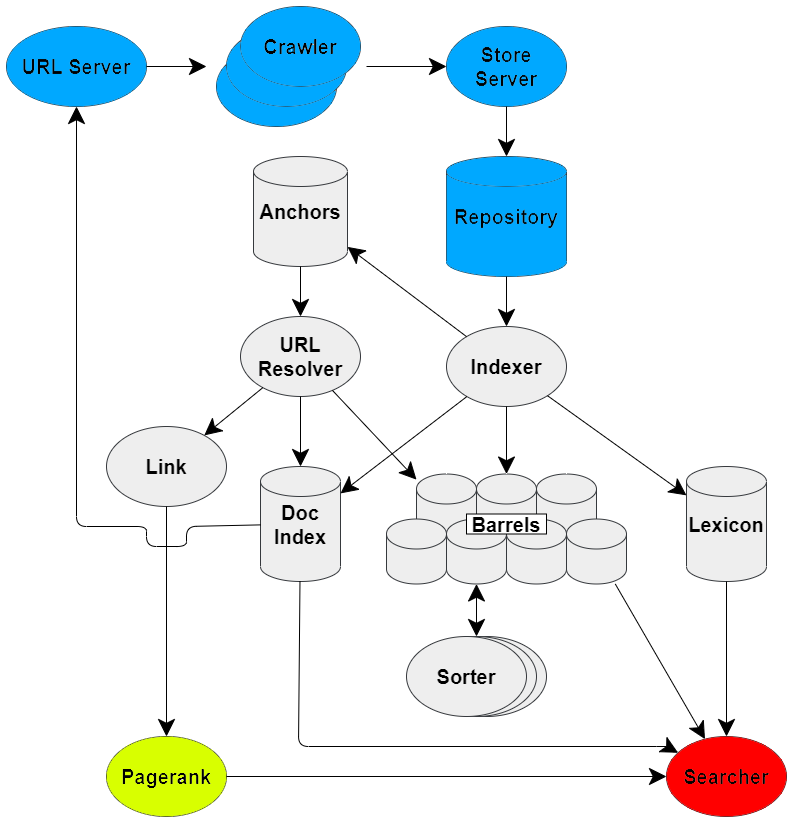
\includegraphics[keepaspectratio, width=7cm]{gambar/google_architecture_filled}
	\caption{\emph{High Level Google Architecture} \citep{brin1998anatomy}}
	\label{gambar:google_architecture_filled}
\end{figure}

Penelitian ini akan merancang dan membangun \textit{search engine} berdasarkan arsitekturnya dengan mengintegrasikan penelitian dari Muhammad Fathan yang berfokus pada perancangan \textit{crawler} menggunakan algoritma \textit{modified similarity based crawling} yang digambarkan sesuai arsitektur pada gambar \ref{gambar:google_architecture_filled} dengan arsiran berwarna biru, penelitian Mohammad Riza yang mengimplementasikan algoritma perangkingan \textit{Google PageRank} yang terdapat pada arsiran kuning, dan penelitian Savira Rahmayanti yang mengembangkan sistem pencarian teks menggunakan metode \textit{TF-IDF} yang terdapat pada arsiran merah.

\section{Rumusan Masalah}
Dari uraian latar belakang di atas, perumusan masalah pada penelitian ini ialah “Bagaimana perancangan arsitektur \textit{search engine} berbasis terminal menggunakan \textit{web crawler}, \textit{page ranking}, dan \textit{document ranking} berbasis \textit{TF IDF}?”

\section{Pembatasan Masalah}
Pembatasan masalah pada penelitian ini antara lain:
\begin{enumerate}
	\item Situs yang menjadi titik awal saat proses \textit{crawling} adalah indosport.com dan curiouscuisiniere.com.
	\item Proses \textit{crawling} dilakukan dengan jangka waktu 1 hari.
	\item Mengkombinasikan metode relevansi pencarian berbasis \textit{TF IDF} dan \textit{Google PageRank}
\end{enumerate}

\section{Tujuan Penelitian}
\begin{enumerate}
	\item Membuat search engine berbasis terminal yang akan menerima \textit{keyword} pencarian dari pengguna menggunakan \textit{crawler}, \textit{Google PageRank}, dan pencarian teks berbasis \textit{TF IDF}.
	\item Membuat \textit{API} dari \textit{REST} \textit{search engine} yang akan dibangun.
\end{enumerate}

\section{Manfaat Penelitian}
\begin{enumerate}
	\item Bagi penulis
		
	Memperluas pengetahuan tentang \textit{search engine}, menambah pengalaman dalam \textit{programming}, memperoleh gelar sarjana di bidang Ilmu Komputer, serta menjadi media untuk penulis dalam mengaplikasikan ilmu yang didapatkan dari kampus.
		
	\item Bagi Program Studi Ilmu Komputer
	 	
	Penelitian ini dapat menjadi pembuka untuk penelitian di masa depan, dan dapat memberikan panduan bagi mahasiswa program studi Ilmu Komputer tentang rancang bangun aplikasi \textit{search engine}.
	
	\item Bagi Universitas Negeri Jakarta
	 	
	Menjadi evaluasi akademik program studi Ilmu Komputer dalam penyusunan skripsi sehingga dapat meningkatkan kualitas pendidikan dan lulusan program studi Ilmu Komputer di Universitas Negeri Jakarta.
	 			
\end{enumerate}


% Baris ini digunakan untuk membantu dalam melakukan sitasi
% Karena diapit dengan comment, maka baris ini akan diabaikan
% oleh compiler LaTeX.
\begin{comment}
\bibliography{daftar-pustaka}
\end{comment}
